
\section{ Enumeration Methodology}


Complex processes must have a standardized methodology that helps us keep our
bearings and avoid omitting any aspects by mistake. Especially with the variety
of cases that the target systems can offer us, it is almost unpredictable how
our approach should be designed. Therefore, most penetration testers follow
their habits and the steps they feel most comfortable and familiar with.
However, this is not a standardized methodology but rather an experience-based
approach.

We know that penetration testing, and therefore enumeration, is a dynamic
process. Consequently, we have developed a static enumeration methodology for
external and internal penetration tests that includes free dynamics and allows
for a wide range of changes and adaptations to the given environment. This
methodology is nested in 6 layers and represents, metaphorically speaking,
boundaries that we try to pass with the enumeration process. The whole
enumeration process is divided into three different levels:
\begin{itemize}
    \item Infrastructure-based enumeration 	
    \item Host-based enumeration 	
    \item OS-based enumeration
\end{itemize}



\begin{figure}
    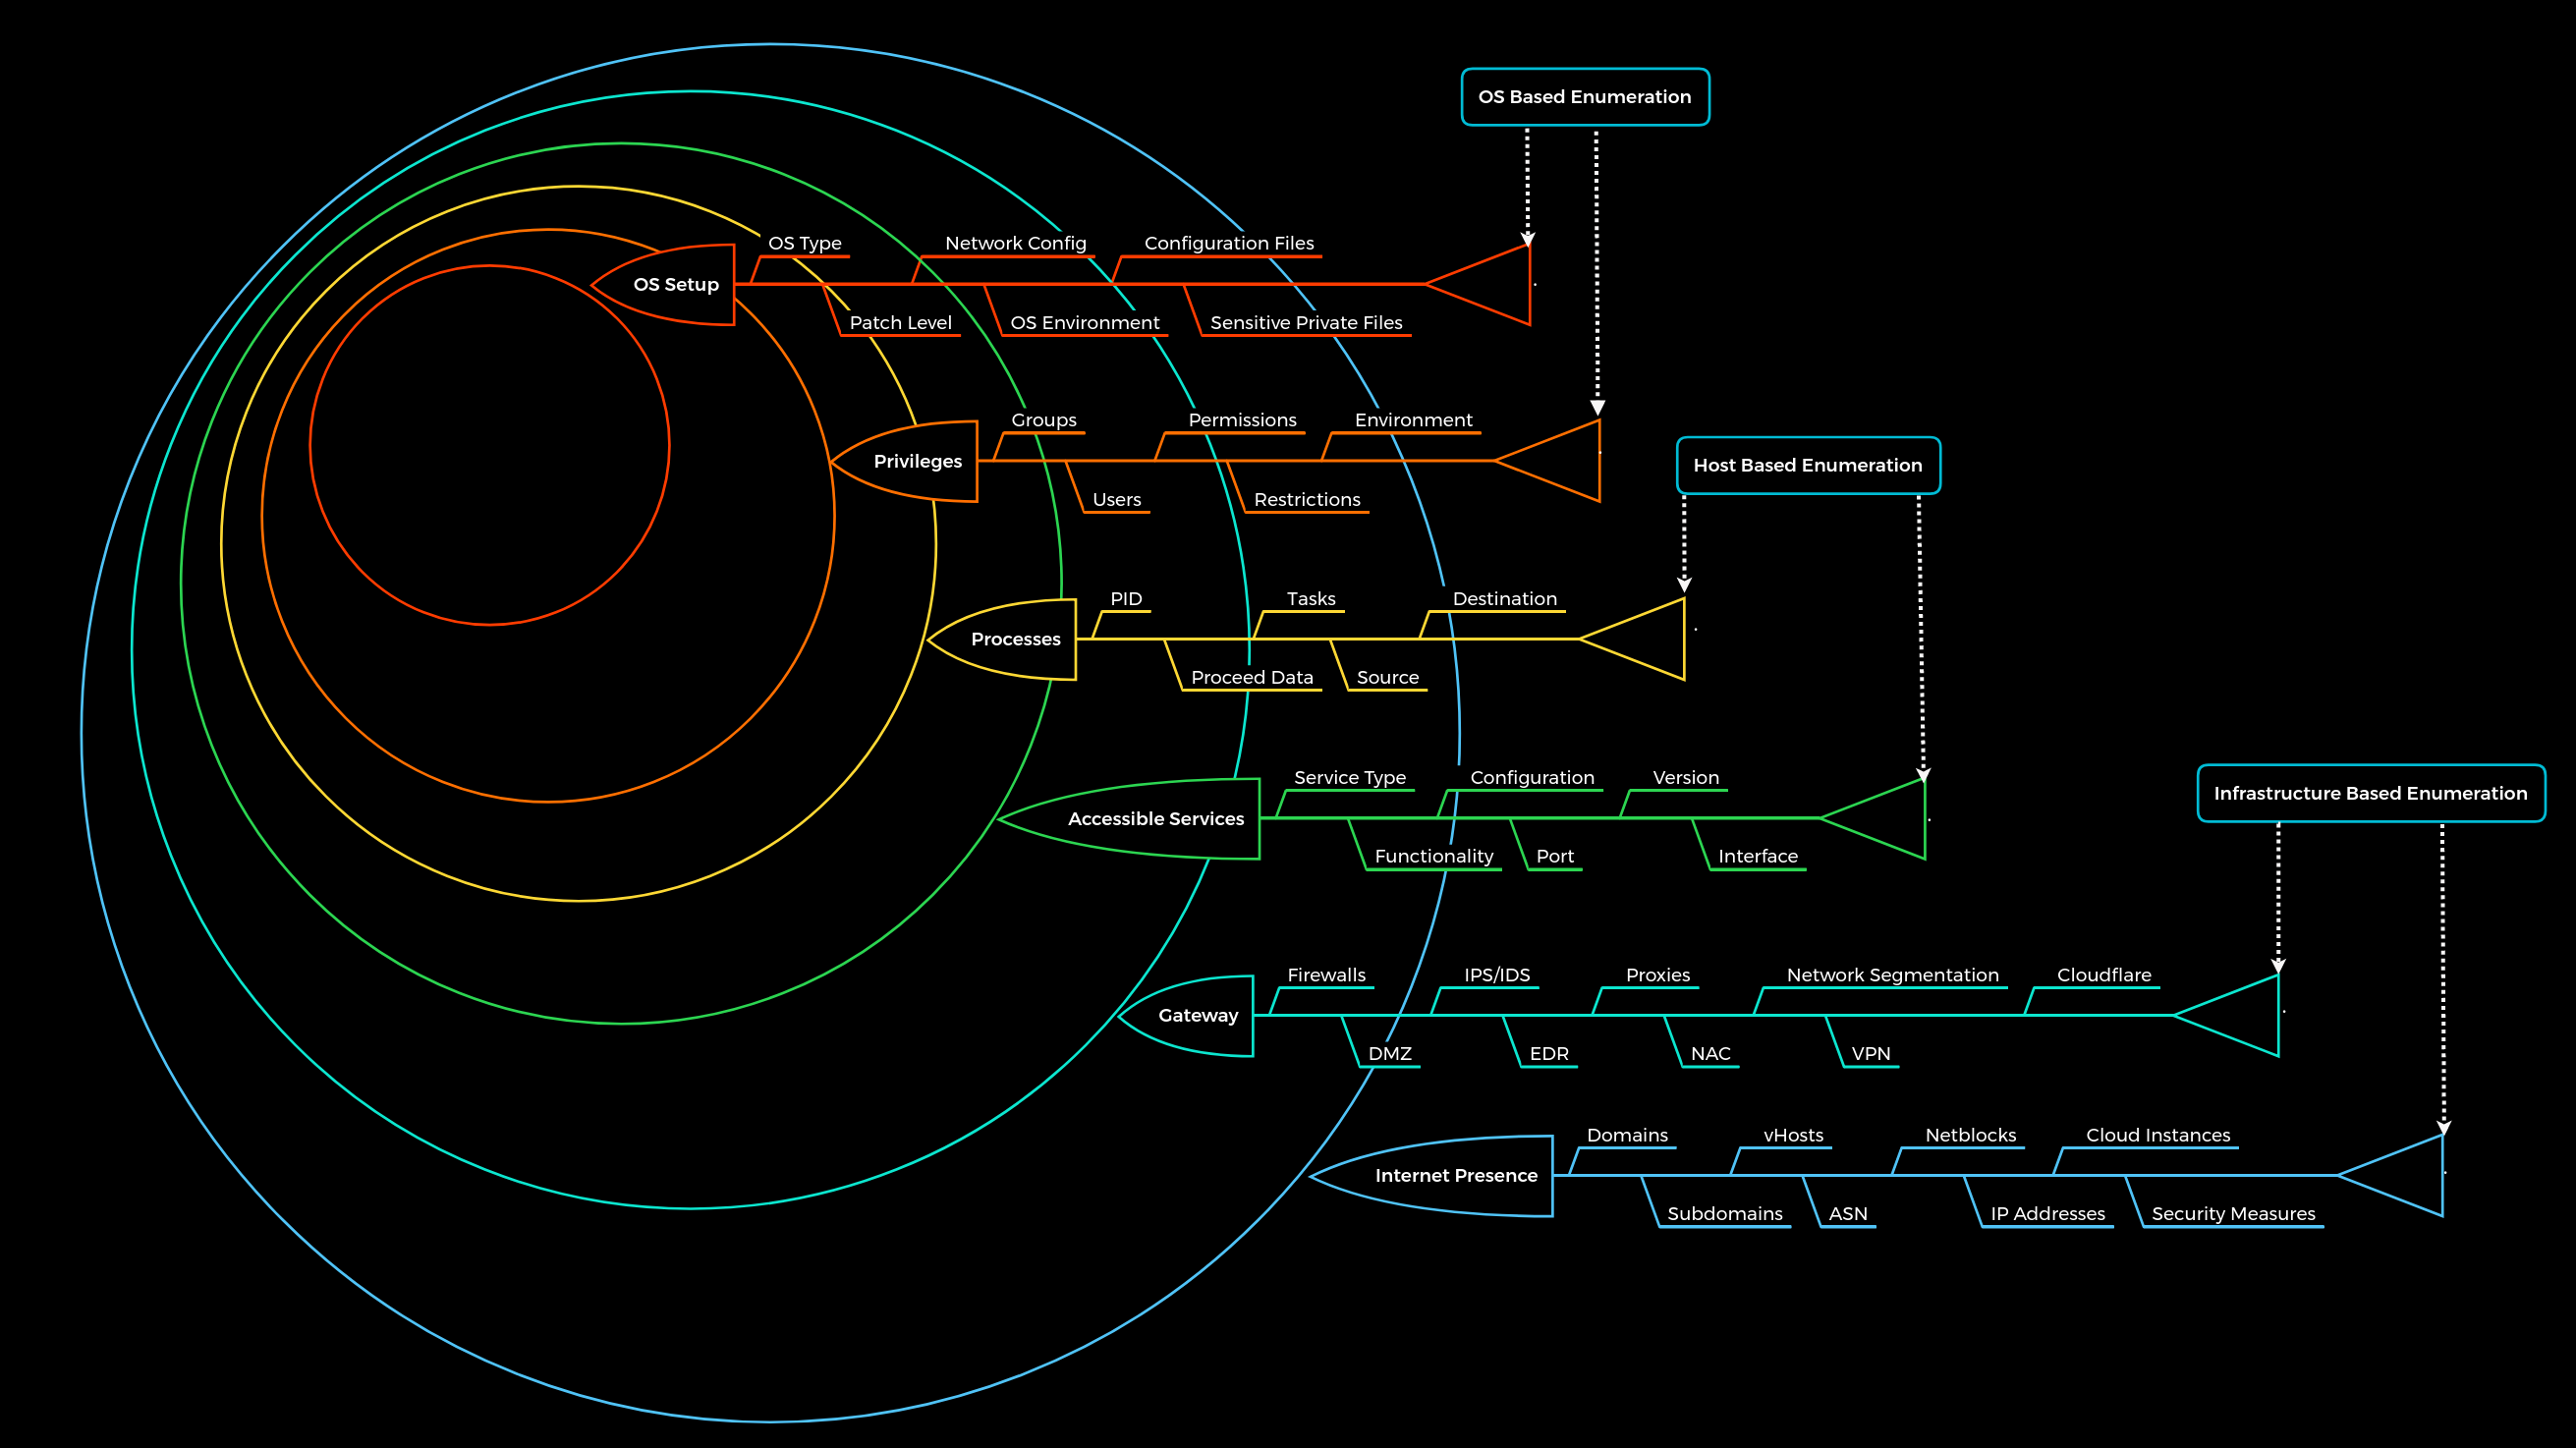
\includegraphics[angle=90,origin=c,width=\linewidth]{recon/intro/images/enum-method.png}
  \caption{Enumeration methodology}
  \label{fig:pentest-process-enum-method}
\end{figure}

Consider these lines as some kind of obstacle, like a wall, for example. What
we do here is look around to find out where the entrance is, or the gap we can
fit through, or climb over to get closer to our goal. Theoretically, it is also
possible to go through the wall headfirst, but very often, it happens that the
spot we have smashed the gap with a lot of effort and time with force does not
bring us much because there is no entry at this point of the wall to pass on to
the next wall.

\begin{itemize}
\item {\bf Internet Presence}: The first layer we have to pass is the
    "Internet Presence" layer, where we focus on finding the targets we can
    investigate. If the scope in the contract allows us to look for additional
    hosts, this layer is even more critical than for fixed targets only. In
    this layer, we use different techniques to find domains, subdomains,
    netblocks, and many other components and information that present the
    presence of the company and its infrastructure on the Internet.

    Identification of internet presence and
    externally accessible infrastructure (Domains, Subdomains, vHosts, ASN,
    Netblocks, IP Addresses, Cloud Instances, Security Measures)
    {\bf The goal of this layer is to identify all possible target systems and
    interfaces that can be tested.}
\item {\bf Gateway}:  	Identify the possible security measures to protect the
    company's external and internal infrastructure (Firewalls, DMZ, IPS/IDS,
    EDR, Proxies, NAC, Network Segmentation, VPN, Cloudflare)
    {\bf The goal is to understand what we are dealing with and what we have to
    watch out for.}
\item {\bf Accessible Services} 	Identify accessible interfaces and services
    that are hosted externally or internally (Service Type, Functionality,
    Configuration, Port, Version, Interface).
    {\bf This layer aims to understand the reason and functionality of the
        target system and gain the necessary knowledge to communicate with it
    and exploit it for our purposes effectively.}
\item {\bf Processes} 	Every time a command or function is executed, data is
    processed, whether entered by the user or generated by the system. This
    starts a process that has to perform specific tasks, and such tasks have at
    least one source and one target.
    {\bf The goal here is to understand these factors and identify the
    dependencies between them.} Identify the internal processes, sources, and
    destinations associated with the services (PID, Proceed Data, Tasks,
    Source, Destination)
\item {\bf Privileges} 	Each service runs through a specific user in a
    particular group with permissions and privileges defined by the
    administrator or the system. These privileges often provide us with
    functions that administrators overlook. This often happens in Active
    Directory infrastructures and many other case-specific administration
    environments and servers where users are responsible for multiple
    administration areas.
    {\bf It is crucial to identify these and understand what is and is not possible with
these privileges.}Identification of the internal permissions and
    privileges to the accessible services (Groups, Users, Permissions,
    Restrictions, Environment)
\item {\bf OS Setup} Here we collect information about the actual operating
    system and its setup using internal access. This gives us a good overview
    of the internal security of the systems and reflects the skills and
    capabilities of the company's administrative teams.
    {\bf The goal here is to see how the administrators manage the systems and what
sensitive internal information we can glean from them.}	Identification of the
internal components and systemsasetup (OS Type, Patch Level, Network config, OS
Environment, Configuration files, sensitive private files \ldots)
\end{itemize}

We can finally imagine the entire penetration test in the form of a labyrinth
where we have to identify the gaps and find the way to get us inside as quickly
and effectively as possible. This type of labyrinth may look something like
this:

\begin{figure}
    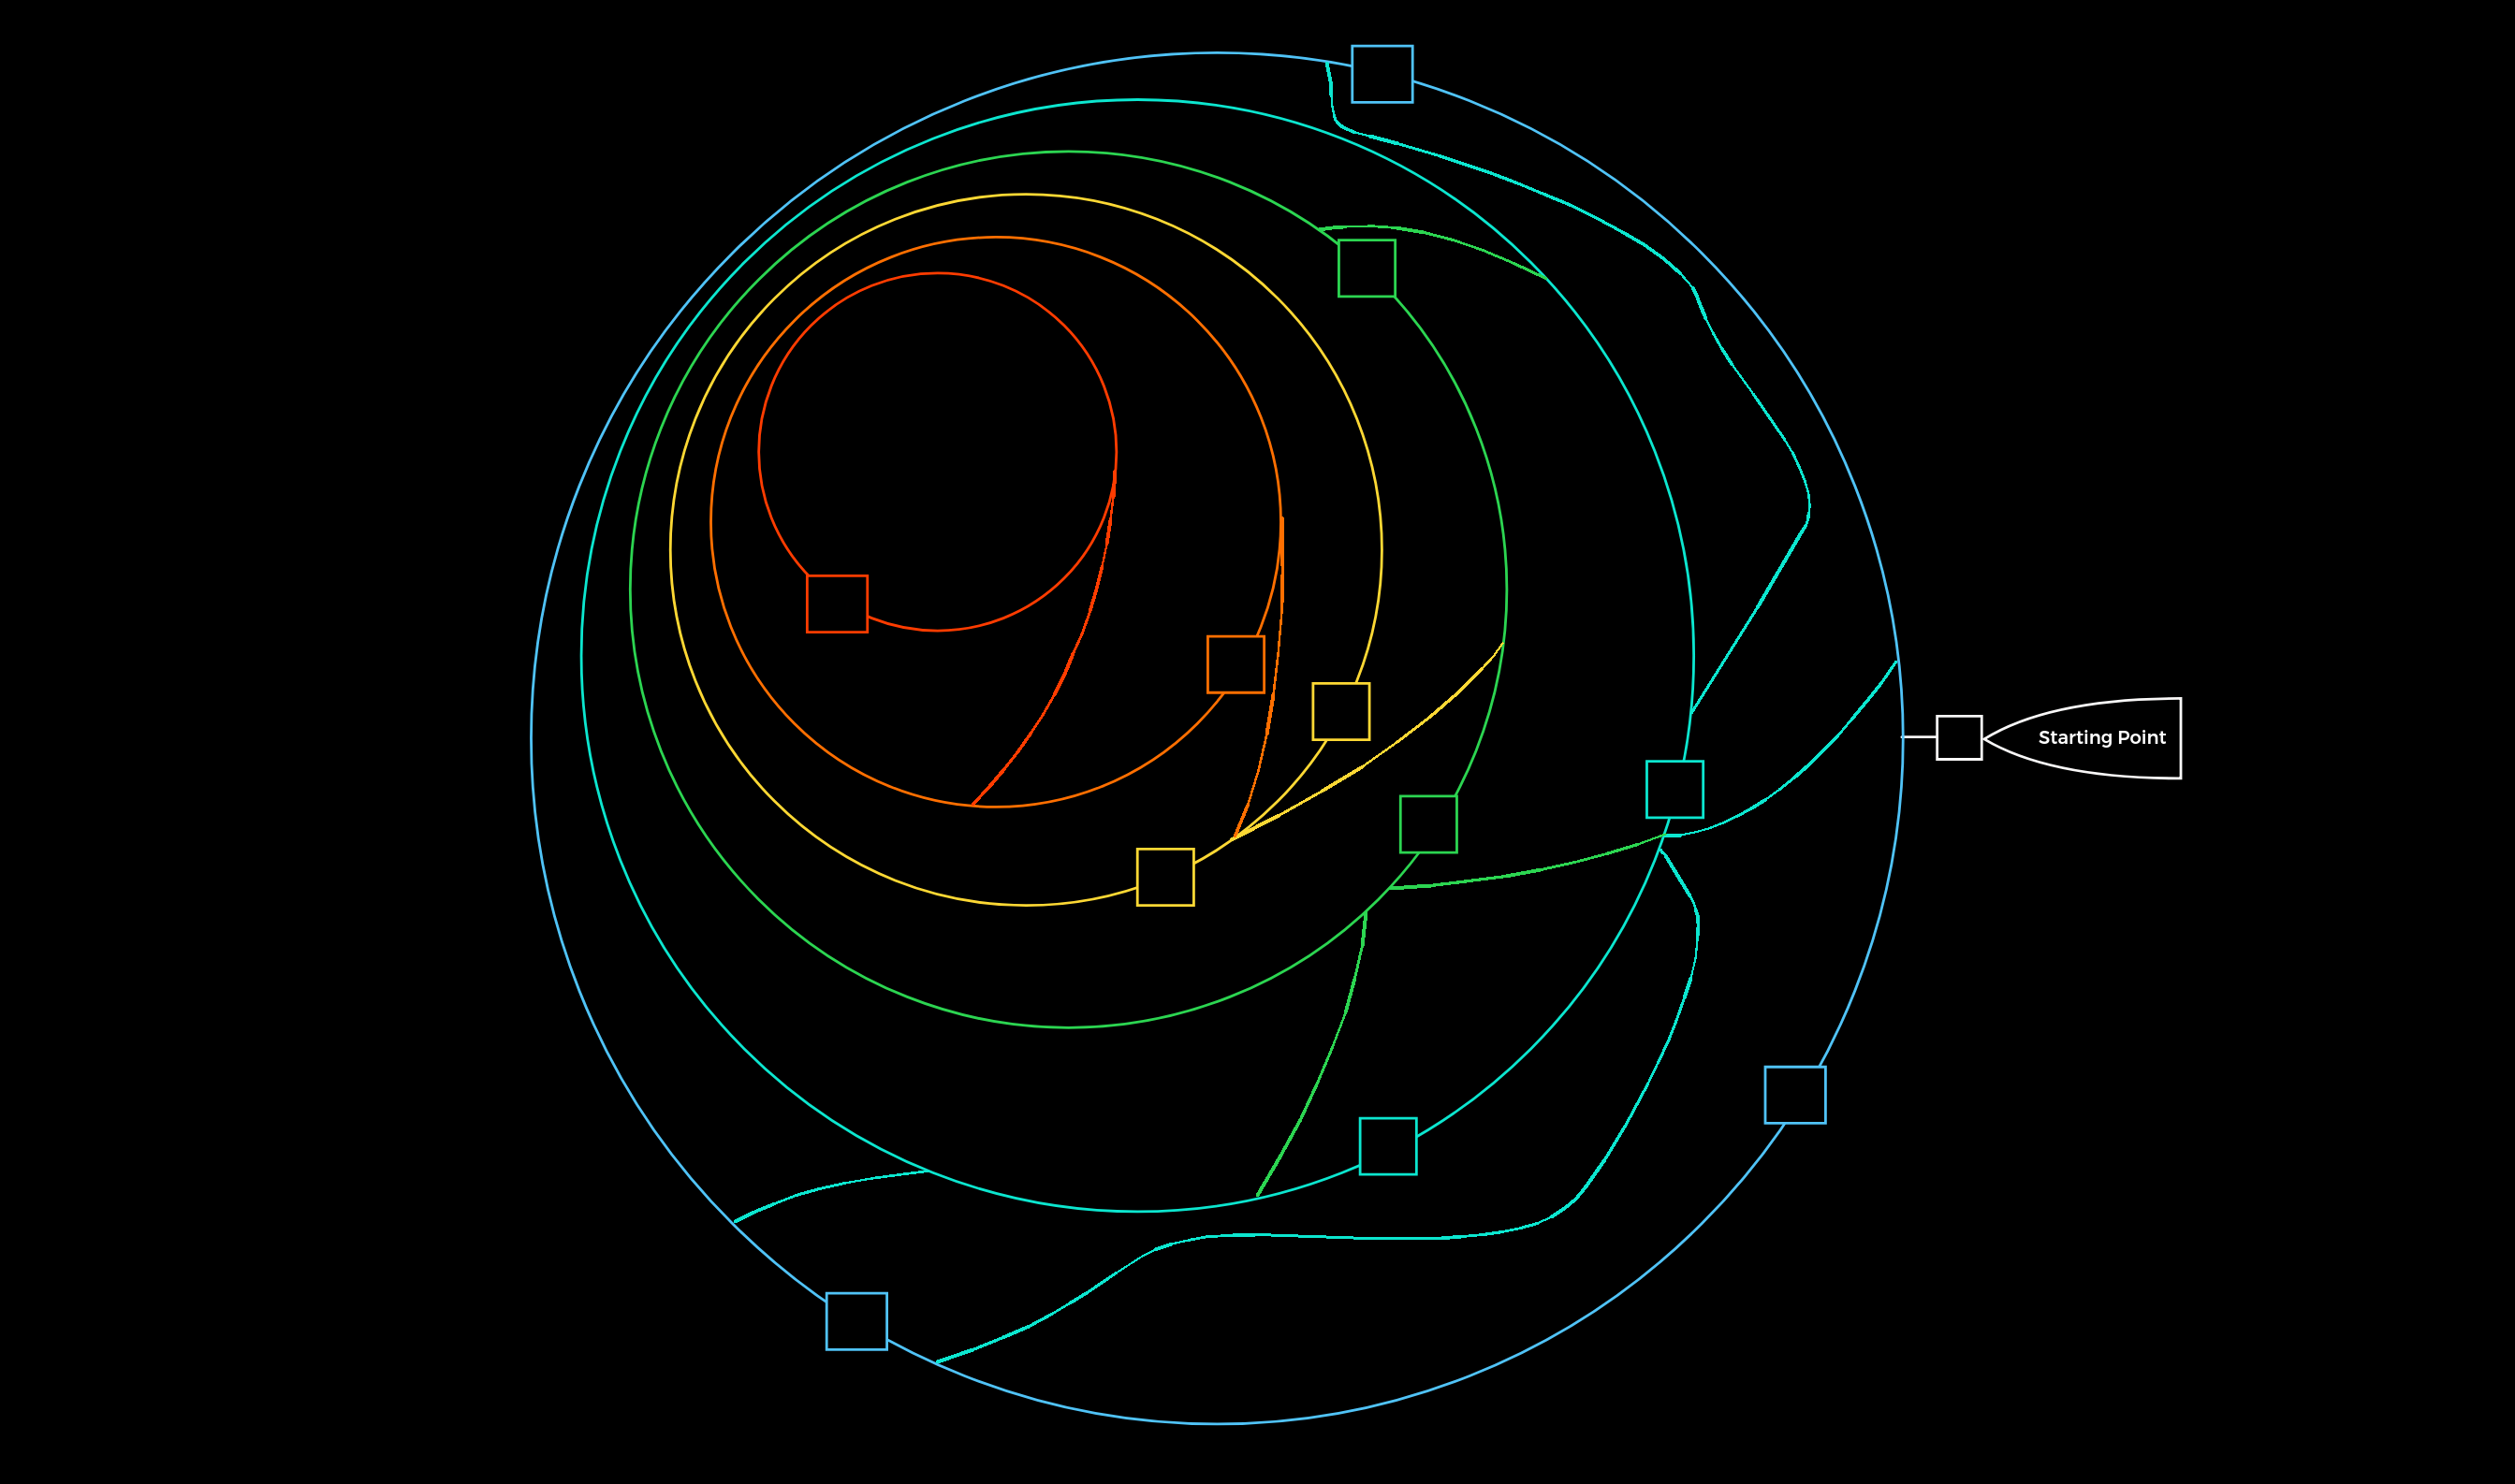
\includegraphics[angle=90,origin=c,width=\linewidth]{recon/intro/images/pentest-labyrinth.png}
  \caption{Pentest labyrinth}
  \label{fig:pentest-pentest-labyrinth}
\end{figure}

As we have probably already noticed, we can see that we will encounter one gap
and very likely several. The interesting and very common fact is that not all
the gaps we find can lead us inside. All penetration tests are limited in time,
but we should always keep in mind that one belief that there is nearly always a
way in. Even after a four-week penetration test, we cannot say 100\% that there
are no more vulnerabilities. Someone who has been studying the company for
months and analyzing them will most likely have a much greater understanding of
the applications and structure than we were able to gain within the few weeks
we spent on the asessment. 
